\chapter{Compiler Architecture and Driver}
\label{chap:architecture}

\section{End-to-End Pipeline Overview}
\label{sec:arch:pipeline}

The NumLang compiler (\texttt{src/compiler.rs}) is structured as an end-to-end, multi-stage pipeline designed for modularity, testability, and deterministic transformation. The pipeline takes raw source text (\texttt{.nl}) and compiles it into either a native standalone executable or executes it directly via an in-process Just-In-Time (JIT) runtime.

Figure~\ref{fig:arch:pipeline} illustrates the seven major transformation stages of the pipeline:

\begin{figure}[h!]
\centering
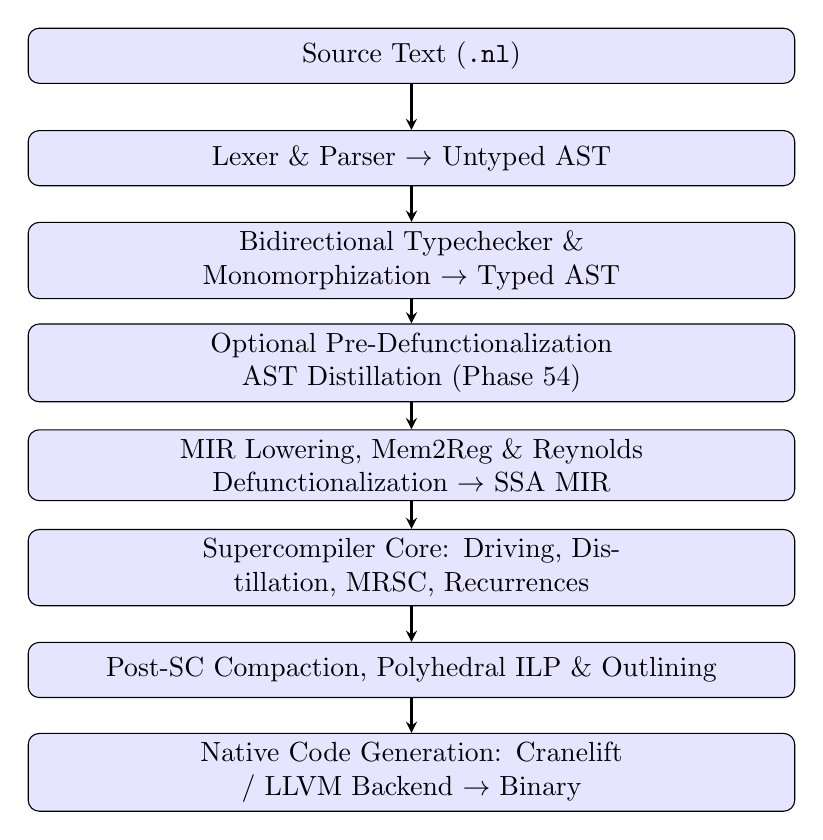
\begin{tikzpicture}[node distance=1.3cm, auto,
    block/.style={rectangle, draw, fill=blue!10, text width=9.5cm, text centered, rounded corners, minimum height=0.7cm},
    arrow/.style={thick, ->, >=stealth}]
    
    \node [block] (source) {Source Text (\texttt{.nl})};
    \node [block, below of=source] (parse) {Lexer \& Parser $\to$ Untyped AST};
    \node [block, below of=parse] (typecheck) {Bidirectional Typechecker \& Monomorphization $\to$ Typed AST};
    \node [block, below of=typecheck] (distill) {Optional Pre-Defunctionalization AST Distillation (Phase 54)};
    \node [block, below of=distill] (mir) {MIR Lowering, Mem2Reg \& Reynolds Defunctionalization $\to$ SSA MIR};
    \node [block, below of=mir] (sc) {Supercompiler Core: Driving, Distillation, MRSC, Recurrences};
    \node [block, below of=sc] (opt) {Post-SC Compaction, Polyhedral ILP \& Outlining};
    \node [block, below of=opt] (codegen) {Native Code Generation: Cranelift / LLVM Backend $\to$ Binary};
    
    \draw [arrow] (source) -- (parse);
    \draw [arrow] (parse) -- (typecheck);
    \draw [arrow] (typecheck) -- (distill);
    \draw [arrow] (distill) -- (mir);
    \draw [arrow] (mir) -- (sc);
    \draw [arrow] (sc) -- (opt);
    \draw [arrow] (opt) -- (codegen);
\end{tikzpicture}
\caption{The end-to-end NumLang compiler pipeline.}
\label{fig:arch:pipeline}
\end{figure}

\section{Command-Line Interface and Driver Flags}
\label{sec:arch:cli}

The compiler CLI driver (\texttt{src/main.rs}) exposes complete control over the metacomputation pipeline through explicit flags:

\begin{itemize}
    \item \texttt{--supercompile}: Activates the supercompilation optimization engine. When omitted, NumLang compiles through the baseline SSA pipeline without metacomputation.
    \item \texttt{--backend <cranelift|llvm>}: Selects the native code generation backend. Cranelift provides $<2$ ms compilation for JIT/AOT development; LLVM provides advanced vectorization and link-time optimization.
    \item \texttt{--opt-level <0|1|2|3>}: Governs backend optimization passes. Level 3 activates aggressive loop unrolling, AVX2 vectorization, and inline threshold expansion.
    \item \texttt{--cache-dir <path>}: Specifies the directory for the content-addressed L2 specialization cache.
    \item \texttt{--incremental}: Enables fine-grained dependency graph tracking and cache reuse on incremental recompilation.
    \item \texttt{--parallel-residualize}: Enables read-write memory independence analysis and generates \texttt{Fork}/\texttt{Join} parallel runtime constructs.
    \item \texttt{--mrsc-exhaustive}: Disables heuristic search and launches an unbounded Iterative Deepening Depth-First Search (IDDFS) over the configuration hypergraph.
    \item \texttt{--emit-termination-proof}: Emits a machine-verifiable JSON termination certificate (\texttt{TerminationWitness}) accompanied by whistle event logs.
    \item \texttt{--supercompile-stats}: Prints a comprehensive performance breakdown detailing whistle firings, knots created, recurrence reductions, and residual code metrics.
\end{itemize}

\section{The BackendCompiler Trait}
\label{sec:arch:backend_trait}

To ensure complete decoupling between intermediate representation transformations and target machine code generation, NumLang defines the \texttt{BackendCompiler} trait in \texttt{src/codegen/backend\_trait.rs}:

\begin{lstlisting}[language=Rust, caption={The BackendCompiler trait in NumLang.}]
pub trait BackendCompiler {
    type Module;
    type Function;
    type Error: std::error::Error;

    fn initialize(&mut self, target_triple: &str) -> Result<(), Self::Error>;
    fn compile_function(&mut self, mir: &MirFunction) -> Result<Self::Function, Self::Error>;
    fn compile_program(&mut self, mir: &MirProgram) -> Result<Self::Module, Self::Error>;
    fn emit_object_file(&self, path: &Path) -> Result<(), Self::Error>;
    fn emit_executable(&self, obj_path: &Path, exe_path: &Path) -> Result<(), Self::Error>;
}
\end{lstlisting}

Both the Cranelift code generator (\texttt{src/codegen/cranelift/}) and the LLVM backend (\texttt{src/codegen/llvm\_backend.rs}) implement this interface identically, ensuring that supercompiler passes remain completely backend-agnostic.

\section{Content-Addressed Specialization Cache}
\label{sec:arch:cache}

Because supercompilation executes expensive symbolic evaluations, compiling large codebases repeatedly from scratch is unacceptable. NumLang deploys a content-addressed, two-level specialization cache (\texttt{src/mir/supercompiler/cache.rs}).

\subsection{Cache Key Derivation}
A cache key must uniquely capture all factors influencing specialization. The key is computed as a SHA-256 cryptographic digest over:
\begin{equation}
\mathcal{K} = \text{SHA-256}\Big(\text{canonicalize}(C_{\text{root}}) \parallel \text{hash}(\text{CalleeTransitiveClosure}) \parallel \text{CompilerVersion}\Big)
\end{equation}
Canonicalization renames all free symbolic variables into a deterministic de Bruijn index sequence, ensuring that identical expressions with differing variable names map to identical cache keys.

\subsection{Two-Level Cache Hierarchy}
\begin{itemize}
    \item \textbf{L1 In-Memory Cache}: A high-speed concurrent hash map storing compiled process tree graphs and residualized MIR functions.
    \item \textbf{L2 On-Disk Cache}: A persistent file store structured with a two-level directory fanout (e.g., \texttt{.cache/sc/3a/7f2b...\dots.json}) to avoid filesystem directory lock contention. Specialization results are serialized as compressed JSON containing residualized MIR and proof witnesses.
\end{itemize}

\section{Tiered JIT and On-Stack Replacement (OSR)}
\label{sec:arch:tiered_jit}

For interactive execution and developer tooling, NumLang includes a multi-tiered runtime engine (\texttt{src/runtime/tier.rs}):

\begin{itemize}
    \item \textbf{Tier 0 (Cold Start)}: When a function is first called, NumLang compiles its unoptimized MIR via Cranelift in under 2 milliseconds, providing instantaneous execution.
    \item \textbf{Profiling Counters}: Tier 0 functions contain invocation and loop back-edge counters. When execution count exceeds the hotness threshold ($\theta = 10,000$), a background compiler task is dispatched to supercompile the function at Tier 1.
    \item \textbf{Tier 1 (Supercompiled Native)}: The function undergoes full symbolic driving, recurrence solving, and distillation.
    \item \textbf{Atomic OSR Swap}: Once Tier 1 compilation finishes, the runtime atomically overwrites the function pointer entry in the global dispatch table using an atomic compare-and-swap (\texttt{AtomicPtr::compare\_exchange}), seamlessly upgrading future invocations without pausing running threads.
\end{itemize}

\section{Incremental Callee Dependency Graph}
\label{sec:arch:incremental}

Delivered in Phase 66, NumLang tracks fine-grained inter-procedural dependencies using an explicit directed acyclic call graph. When a source file is edited:
\begin{enumerate}
    \item The compiler computes the set of modified function ASTs.
    \item The dependency graph performs reverse reachability analysis, identifying the exact transitive closure of callers whose specialization states could be affected.
    \item All unaffected functions (typically $>80\%$ of the codebase in standard leaf-function edits) bypass the supercompiler entirely and load pre-compiled residuals directly from the L2 cache.
\end{enumerate}
This delivers interactive recompilation speeds comparable to traditional single-pass compilers while retaining global metacomputation power.

\section{Comprehensive CLI Options Reference Manual}
\label{sec:arch:cli_manual}

The NumLang driver binary (\texttt{numlang}) provides a unified CLI interface:

\begin{lstlisting}[caption={Command-Line Interface Flags of the NumLang Compiler.}]
numlang 0.1.0 (Advanced SSA Metacompiler)
USAGE:
    numlang [OPTIONS] <INPUT_FILE> [SUBCOMMAND]

FLAGS:
    --supercompile              Enable whole-program supercompilation pipeline
    --backend <BACKEND>         Select codegen backend: cranelift (default) | llvm
    --opt-level <LEVEL>         Optimization level (0, 1, 2, 3)
    --cache-dir <DIR>           Directory path for L2 persistent specialization cache
    --incremental               Enable callee call-graph incremental cache reuse
    --parallel-residualize      Enable memory independence analysis and Fork/Join codegen
    --mrsc-exhaustive           Activate unbounded IDDFS MRSC configuration oracle
    --emit-termination-proof    Emit cryptographic JSON TerminationWitness certificates
    --supercompile-stats        Print detailed metacomputation metrics upon completion
    -h, --help                  Print help information
    -V, --version               Print version information

SUBCOMMANDS:
    run                         Compile and immediately execute in-process via JIT
    build                       Compile to standalone native machine executable
    check                       Execute lexical, parsing, and typechecking verification
    clean                       Flush compiler L1/L2 specialization cache stores
\end{lstlisting}
